\begin{figure}
\centering
  \begin{tabular}{c}
  
%%%%% expt1  
  
  \begin{subfigure}{0.45\textwidth}
 \tabl{c}{\scalebox{0.8}{\begin{tikzpicture}
      \begin{axis}[
	xlabel={timestep},
	ylabel={Cumulative regret},
       clip mode=individual,grid,grid style={gray!30},
  legend style={at={(0.5,-0.2)},anchor=north,legend columns=3} ]  
  % UCB    

\addplot table[x index=0,y index=1,col sep=tab,each nth point={10}] {results/Expt1/UCB_Vcomp_subsampled.txt};
\addplot table[x index=0,y index=1,col sep=tab,each nth point={10}] {results/Expt1/DMEDcomp_subsampled.txt};
\addplot table[x index=0,y index=1,col sep=tab,each nth point={10}] {results/Expt1/KLUCBcomp_subsampled.txt};
\addplot table[x index=0,y index=1,col sep=tab,each nth point={10}] {results/Expt1/MOSScomp_subsampled.txt};
\addplot table[x index=0,y index=1,col sep=tab,each nth point={10}] {results/Expt1/UCB1comp_subsampled.txt};
\addplot table[x index=0,y index=1,col sep=tab,each nth point={10}] {results/Expt1/TScomp_subsampled.txt};
\addplot table[x index=0,y index=1,col sep=tab,each nth point={10}] {results/Expt1/clUCBcomp_subsampled.txt};
      \legend{UCB-V,DMED,KL-UCB,MOSS,UCB1,TS,ClusUCB(p=4)}
      \end{axis}
      \end{tikzpicture}}\\}
			\caption{Experiment $1$: $20$ Bernoulli-distributed arms with $r_{i_{a_{i}\neq a^{*}}}=0.07$ and $r^{*}=0.1$.}
  \label{fig:1}
  \end{subfigure}
	\\
	%%%%%%% Expt 2
	  \begin{subfigure}{0.45\textwidth}
 \tabl{c}{\scalebox{0.8}{\begin{tikzpicture}
      \begin{axis}[
	xlabel={timestep},
	ylabel={Cumulative regret},
       clip mode=individual,grid,grid style={gray!30},
  legend style={at={(0.5,-0.2)},anchor=north,legend columns=3} ]
      % UCB
\addplot table[x index=0,y index=1,col sep=tab,each nth point={10}] {results/Expt2/clUCBCcomp_subsampled.txt};
\addplot table[x index=0,y index=1,col sep=tab,each nth point={10}] {results/Expt2/clUCBNCcomp_subsampled.txt};
\addplot table[x index=0,y index=1,col sep=tab,each nth point={10}] {results/Expt2/Med_Elimcomp_subsampled.txt};
\addplot table[x index=0,y index=1,col sep=tab,each nth point={10}] {results/Expt2/UCB_Improvedcomp_subsampled.txt};
\addplot table[x index=0,y index=1,col sep=tab,each nth point={10}] {results/Expt2/MOSScomp_subsampled.txt};
\addplot table[x index=0,y index=1,col sep=tab,each nth point={10}] {results/Expt2/UCB1comp_subsampled.txt};
      \legend{ClusUCB (p=20), ClusUCB (p=1), Med-Elim,UCB-Improved,MOSS,UCB1}
      \end{axis}
      \end{tikzpicture}}\\}
			\caption{Experiment $2$: $100$ Gaussian-distributed arms with $r_{i_{a_{i}\neq a^{*}:1-33}}=0.01$, $r_{i_{a_{i}\neq a^{*}:34-99}}=0.06$ and $r^{*}_{i=100}=0.1$.}
  \label{fig:2}
  \end{subfigure}
	\\
	%%%%%%% Expt 3
	  \begin{subfigure}{0.45\textwidth}
 \tabl{c}{\scalebox{0.8}{\begin{tikzpicture}
      \begin{axis}[
	xlabel={Arms},
	ylabel={Cumulative regret},
       clip mode=individual,grid,grid style={gray!30},
  legend style={at={(0.5,-0.2)},anchor=north,legend columns=-1} ]
      % UCB
\addplot table[x index=0,y index=1,col sep=tab] {results/Expt3/clUCB20_400.txt};
\addplot table[x index=0,y index=1,col sep=tab] {results/Expt3/MOSS20_400.txt};
      \legend{ClusUCB,MOSS}
      \end{axis}
      \end{tikzpicture}}\\}
			\caption{Experiment $3$: $20$ to $400$ Bernoulli-distributed arms with $r_{i_{a_{i}\neq a^{*}}}=0.05$ and $r^{*}=0.1$.}
  \label{fig:3}
  \end{subfigure}
  \end{tabular}
\caption{Cumulative regret for various bandit algorithms on three stochastic K-armed bandit environments. 
}
\label{fig:karmed}
\end{figure}

\begin{figure}
\centering
  \begin{tabular}{c}
  \begin{subfigure}{0.45\textwidth}
 \tabl{c}{\scalebox{0.8}{\begin{tikzpicture}
      \begin{axis}[
	xlabel={timestep},
	ylabel={Cumulative regret},
       clip mode=individual,grid,grid style={gray!30},
  legend style={at={(0.5,-0.2)},anchor=north, legend columns=2} ]
      % UCB
\addplot table[x index=0,y index=1,col sep=tab,each nth point={10}] {results/Expt4/clUCB1comp_subsampled.txt};
\addplot table[x index=0,y index=1,col sep=tab,each nth point={10}] {results/Expt4/clUCB2comp_subsampled.txt};
\addplot table[x index=0,y index=1,col sep=tab,each nth point={10}] {results/Expt4/clUCB3comp_subsampled.txt};
\addplot table[x index=0,y index=1,col sep=tab,each nth point={10}] {results/Expt4/MOSScomp_subsampled.txt};
\addplot table[x index=0,y index=1,col sep=tab,each nth point={10}] {results/Expt4/clUCB4comp_subsampled.txt};
\addplot table[x index=0,y index=1,col sep=tab,each nth point={10}] {results/Expt4/clUCB5comp_subsampled.txt};
\addplot table[x index=0,y index=1,col sep=tab,each nth point={10}] {results/Expt4/TScomp_subsampled.txt};
      \legend{ClusUCB(1A),ClusUCB(4B),ClusUCB(10B),MOSS,ClusUCB(5S),ClusUCB(10S),TS}
      %\legend{ClusUCB (NC, p=1),ClusUCB (C, p=4),ClusUCB(C, p=10) ,MOSS, ClusUCB(C, p=5, NAE), ClusUCB(C, p=10, NAE)}
      %\legend{ClusUCB(1,A),ClusUCB(4,B),ClusUCB(10,B), MOSS,ClusUCB(5,S), ClusUCB(10,A)}
      \end{axis}
      \end{tikzpicture}}\\}
			\caption{Experiment $4$: ClusUCB for various $p$. ClusUCB(1A)= $\lbrace$ p=$1$,Only Arm Elimination $\rbrace$, ClusUCB(4B)=$\lbrace$ p=$4$, Both Arm and Cluster Elimination$\rbrace$, ClusUCB(5S)=$\lbrace$ p=$5$, Only Cluster Elimination$\rbrace$. }
  \label{Fig:variousClus}
  \end{subfigure}
  \end{tabular}

\end{figure}

%\begin{figure}[!tbp]
%\label{fig:1}
%\begin{minipage}[b]{0.5\textwidth}
%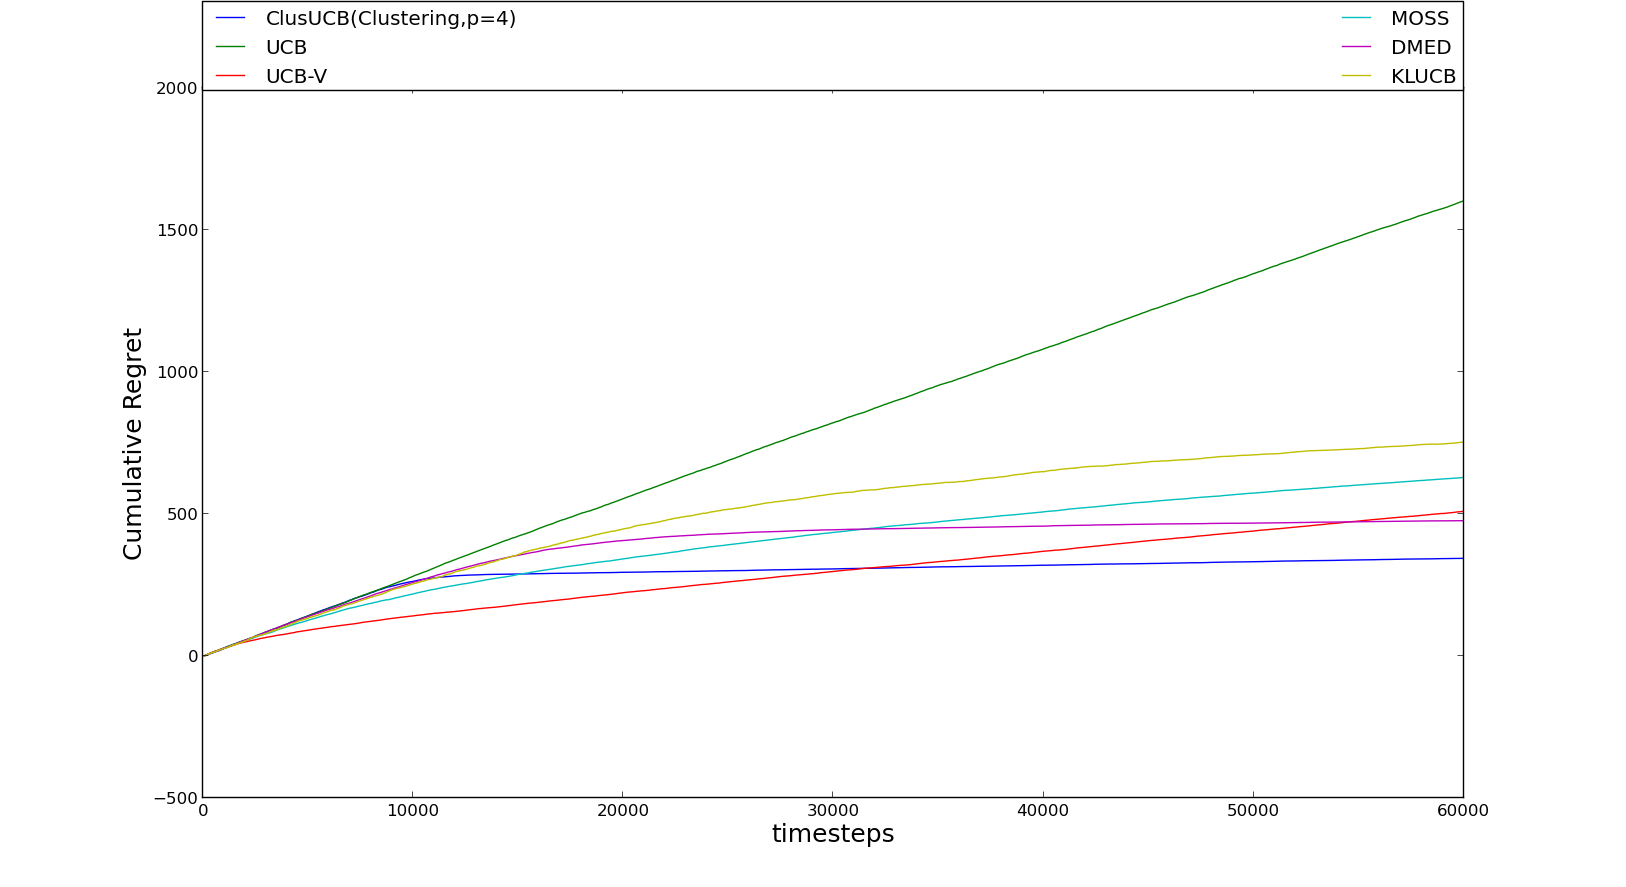
\includegraphics[width=\textwidth]{img/ClusUCB_variousAlgo.png}
%
%\caption{Experiment 1: Regret for various Algorithms. $T=60000$}
%\end{minipage}
%\end{figure}
%
%\hspace{0.1em}
%
%\begin{figure}[!tbp]
%\label{fig:2}
%\begin{minipage}[b]{0.5\textwidth}
%
%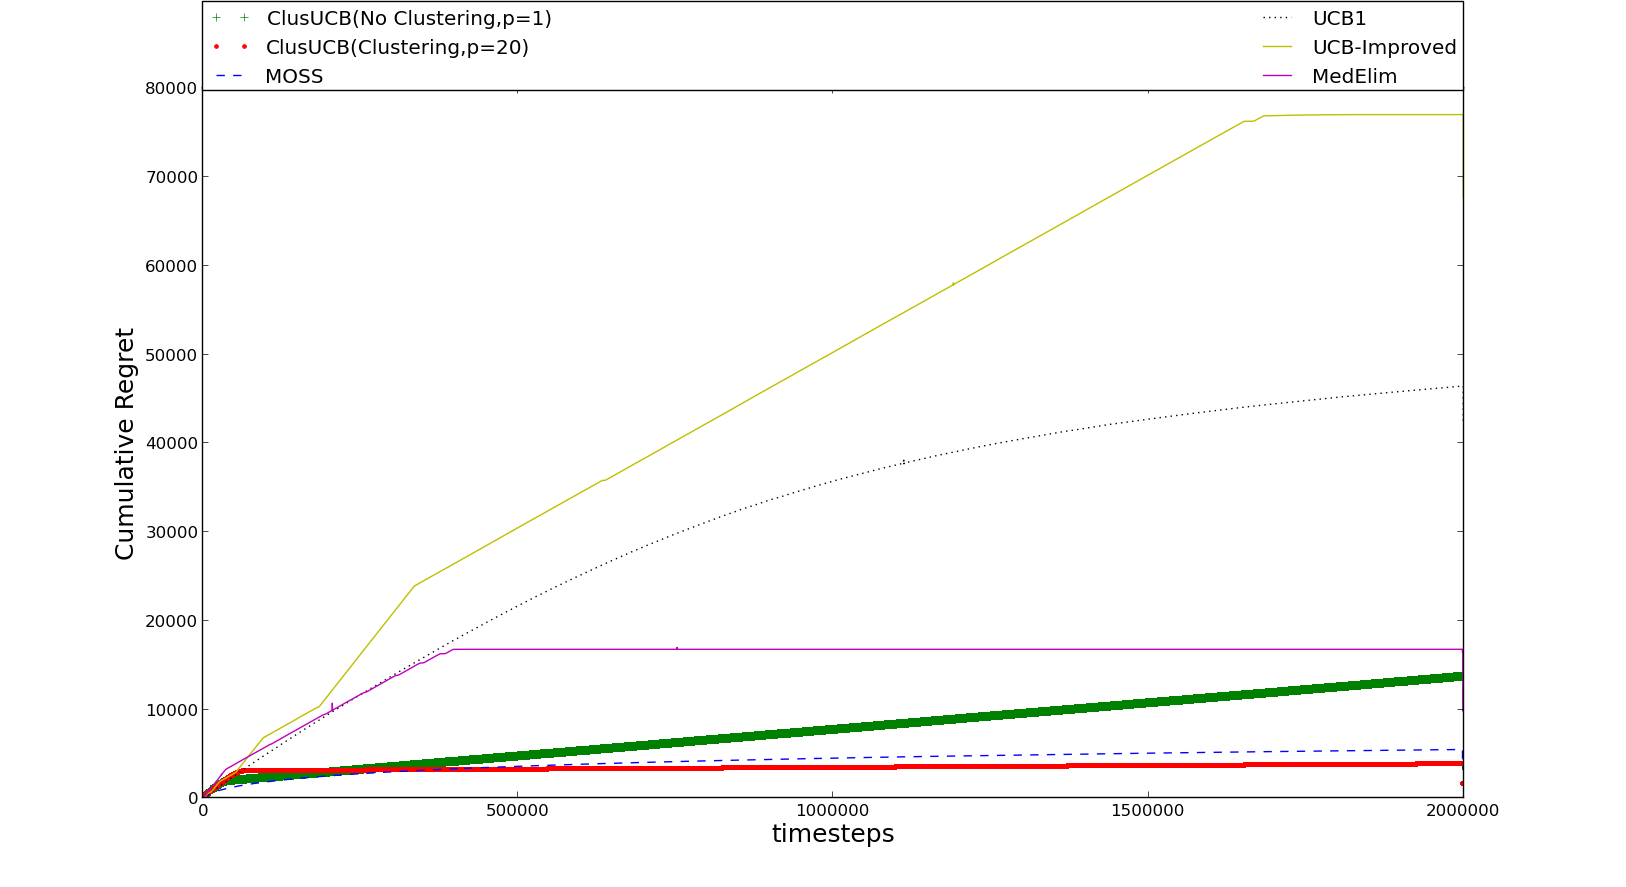
\includegraphics[width=\textwidth]{img/clusUCB_variousAlgo(expt2)_Final.png}
%\caption{Experiment 2: Regret for various Algorithms. $T=2\times 10^{6}$}
%\end{minipage}
%\end{figure}
%
%\hspace{0.1em}
%
%\begin{figure}[!tbp]
%\label{fig:3}
%\begin{minipage}[b]{0.5\textwidth}
%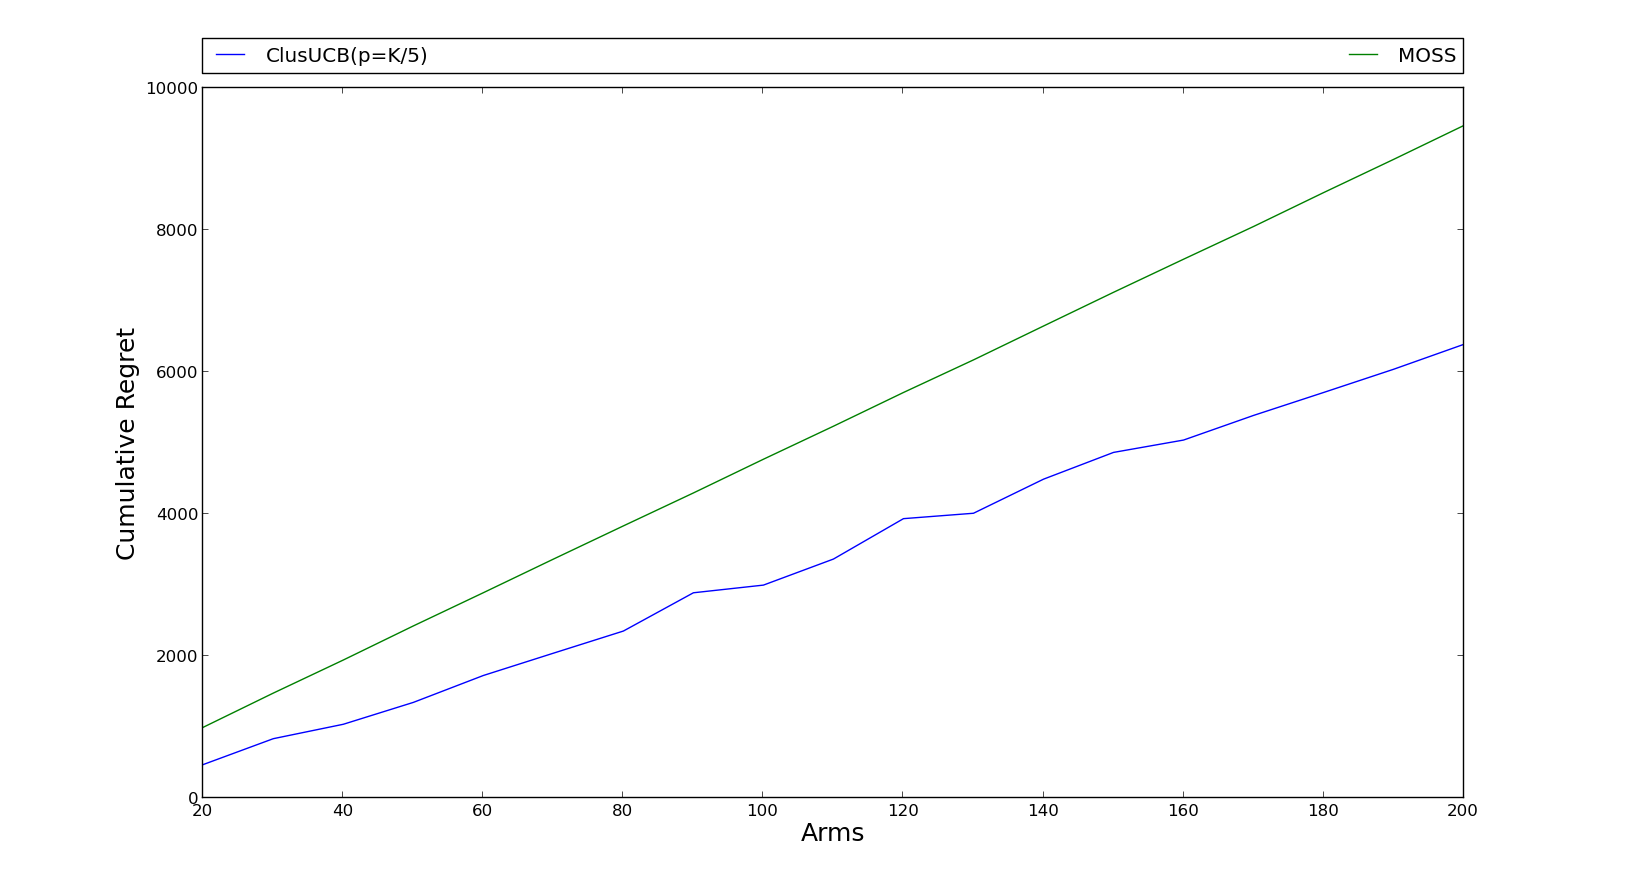
\includegraphics[width=\textwidth]{img/clUCB_MOSS_expt3.png}
%\caption{Experiment 3: Regret Growth for ClusUCB and MOSS . $T=10^{5} + K^{2}\times 10^{4}$ for $K=20$ to $200$}
%\end{minipage}
%\end{figure}
%
%\hspace{0.1em}
%


%In the stochastic bandit literature there are several powerful algorithms with and without proven regret bounds. Algorithms like $\epsilon$-greedy(\cite{sutton1998reinforcement}) or softmax(\cite{sutton1998reinforcement}) or UCB-Tuned(\cite{auer2002finite}) has no proven regret bounds. Again algorithms like UCB-$\delta$(\cite{abbasi2011improved}) with proven regret bound better than UCB1  falls within the realm of fixed confidence setting whereas one has to provide the probability of error $\delta$. We also make a distinction between frequentist based approach like the UCB algorithms and the Bayesian approach like the Thompson Sampling(\cite{agrawal2011analysis}). 
For the sake of performance comparison using cumulative regret as the metric, we implement the following algorithms:  KL-UCB\cite{garivier2011kl}, DMED\cite{honda2010asymptotically}, MOSS\cite{audibert2009minimax}, UCB1\cite{auer2002finite}, UCB-Improved\cite{auer2010ucb}, Median Elimination\cite{even2006action}, Thompson Sampling(TS)\cite{agrawal2011analysis} and UCB-V\cite{audibert2009exploration}\footnote{The implementation for KL-UCB and DMED are taken from \cite{CapGarKau12}.}.

The parameters of ClusUCB algorithm are set as follows: $\psi=\log T$, $\rho_{s}=\dfrac{1}{2^{2m+1}}$ and $\rho_{a}=\dfrac{1}{2^{4m+1}}$ for $m=0,1,...,\big \lfloor \dfrac{1}{2}\log_{2} \dfrac{T}{e}\big\rfloor$. So in all the experiments $\rho_{a}$ and $\rho_{s}$ are initialized to $1$ and then reduced after every round. By this definition of $\rho_{a},\rho_{s}$ we have made sure that their value always remain bounded $\in(0,1]$. When $K$ is large and $p$ is small it is advantageous to run $\rho_{a} < \rho_{s}$(see Corollary \ref{Result:Corollary:2}) because this will aggressively eliminate arms within cluster while cluster elimination will be more conservative since each cluster will contain a large number of arms it should be eliminated less aggressively. 
The first experiment is conducted over a testbed of $20$ arms for the test-cases involving Bernoulli reward distribution with expected rewards of the arms $r_{i_{a_{i}\neq a^{*}}}=0.07$ and $r^{*}=0.1$. These type of cases are frequently encountered in web-advertising domain. The horizon $T$ is set to $60000$ and the number of clusters $p$ for ClusUCB is set to $4$. The regret is averaged over $100$ independent runs and is shown in Figure \ref{fig:1}. 
ClusUCB, MOSS, UCB1, UCB-V, KL-UCB, TS and DMED are run in this experimental setup and we observe that ClusUCB performs better than all the aforementioned algorithms. Because of the short horizon $T$, we do not implement UCB-Improved and Median Elimination on this test-case. We also see that in this case the cumulative regret of ClusUCB and TS are very close to each other though ClusUCB is slightly better.

The second experiment is conducted over a testbed of $100$ arms involving Gaussian reward distribution with expected rewards of the arms $r_{i_{a_{i}\neq a^{*}:1-33}}=0.01$, $r_{i_{a_{i}\neq a^{*}:34-99}}=0.06$ and $r^{*}_{i=100}=0.1$ with variance set at $\sigma = 0.3,\forall i\in A$. The horizon $T$ is set for a large duration of $2\times 10^{6}$ and the number of clusters $p=20$. The regret is averaged over $100$ independent runs and is shown in Figure \ref{fig:2}. In this case, in addition to ClusUCB, we also show the performance of no-clustering version of ClusUCB algorithm (i.e., $p=1$).   From the results sin Figure \ref{fig:2}, we observe that ClusUCB with $p=20$ outperforms ClusUCB with $p=1$ as well as MOSS, UCB1, UCB-Improved and Median-Elimination($\epsilon=0.03,\delta=0.1$). We also observed that the ClusUCB variant that uses only  the arm elimination condition in Algorithm \ref{alg:clusucb} performs worse than the variant that employs cluster and arm elimination conditions. We also see that in this testbed UCB-Improved performs the worst and it confirms our assumption 
that it spends too much pulls in the initial exploration.

The third experiment is conducted over a testbed of $20-400$(interval of $10$) arms with Bernoulli reward distribution, where the expected rewards of the arms are $r_{i_{a_{i}\neq a^{*}}}=0.05$ and $r^{*}=0.1$. The horizon $T$ is set to $10^{5} + K^{2}\times 10^{4}$ and the number of arms are increased from $K=20$ to $200$. ClusUCB is run with $p=K/5$. The regret is averaged over $500$ independent runs and is shown in Figure \ref{fig:3}. We report the performance of MOSS and ClusUCB only over this setup. From the results in Figure \ref{fig:3}, it is evident that the growth of regret for ClusUCB is lower than MOSS. 

The fourth experiment is performed over a testbed having $20$ Bernoulli-distributed arms with $r_{i_{:{a_{i}\neq a^{*}}}}=0.06,\forall i\in A$ and $r^{*}=0.1$. In Figure \ref{Fig:variousClus}, we report the results with $T=60000$ averaged over $100$ independent runs for ClusUCB with  $p=\lbrace 1,4,10\rbrace$. Also, in this experiment we take $\psi = 1.0$ just to make sure that we only see the effect of arm and cluster elimination parameters on clustering. Since now the exploration is really low, there is a greater number of errors committed by ClusUCB-AE that is ClusUCB(p=1). Two other benchmark algorithms are considered here, MOSS which is one of our main competitors and TS which has performed near equivalently in experiment $1$(see Fig \ref{fig:1}). In this case we see that, since $\rho_{a}$ is decreased very fast, the optimal arm $a^{*}$ gets eliminated most of the time for no clustering $p=1$. While a balance of $p,\rho_{a}$ and $\rho_{s}$ gives a much better result. ClusUCB with $p=4$ and $10$ perform better than MOSS, while $p=1$ with just arm elimination does not converge and $p=5,10$ with just Cluster elimination and no arm elimination also does not converge. In this test-bed we see that ClusUCB($p=4$) beats TS. As proved in Proposition \ref{proofSketch:Prop:2}, regret for using just cluster elimination is higher than using just arm elimination. A balance of cluster and arm elimination works best. For using just cluster elimination in ClusUCB($\sqrt{\log K}<p\leq \dfrac{K}{2}$) we stop when we are left with one cluster and output the max payoff arm of that cluster.

%We set $\psi=1$, $\rho_{s}=\frac{1}{2^{m+1}}$ and $\rho_{a}=\frac{1}{2^{2m+1}}$.

%The jumps in the graph for ClusUCB happens because of the error(eliminating optimal arm) and the margin of error(in red) is also shown in the graph. 
%\todos{I did not see this jump in the txt files shared for Expt 3}
